\documentclass{article}

\usepackage{graphicx}
\usepackage{tikz}
\usepackage{tikzsymbols}
\usetikzlibrary{calc,patterns,shapes.geometric}
\pagestyle{empty}
\usepackage[margin=0pt]{geometry}
\geometry{papersize={14in,12in}}

\def\centerarc[#1](#2)(#3:#4:#5){\draw[#1] ($(#2)+({#5*cos(#3)},{#5*sin(#3)})$) arc (#3:#4:#5);}

\begin{document}
	\begin{figure}
		\centering
		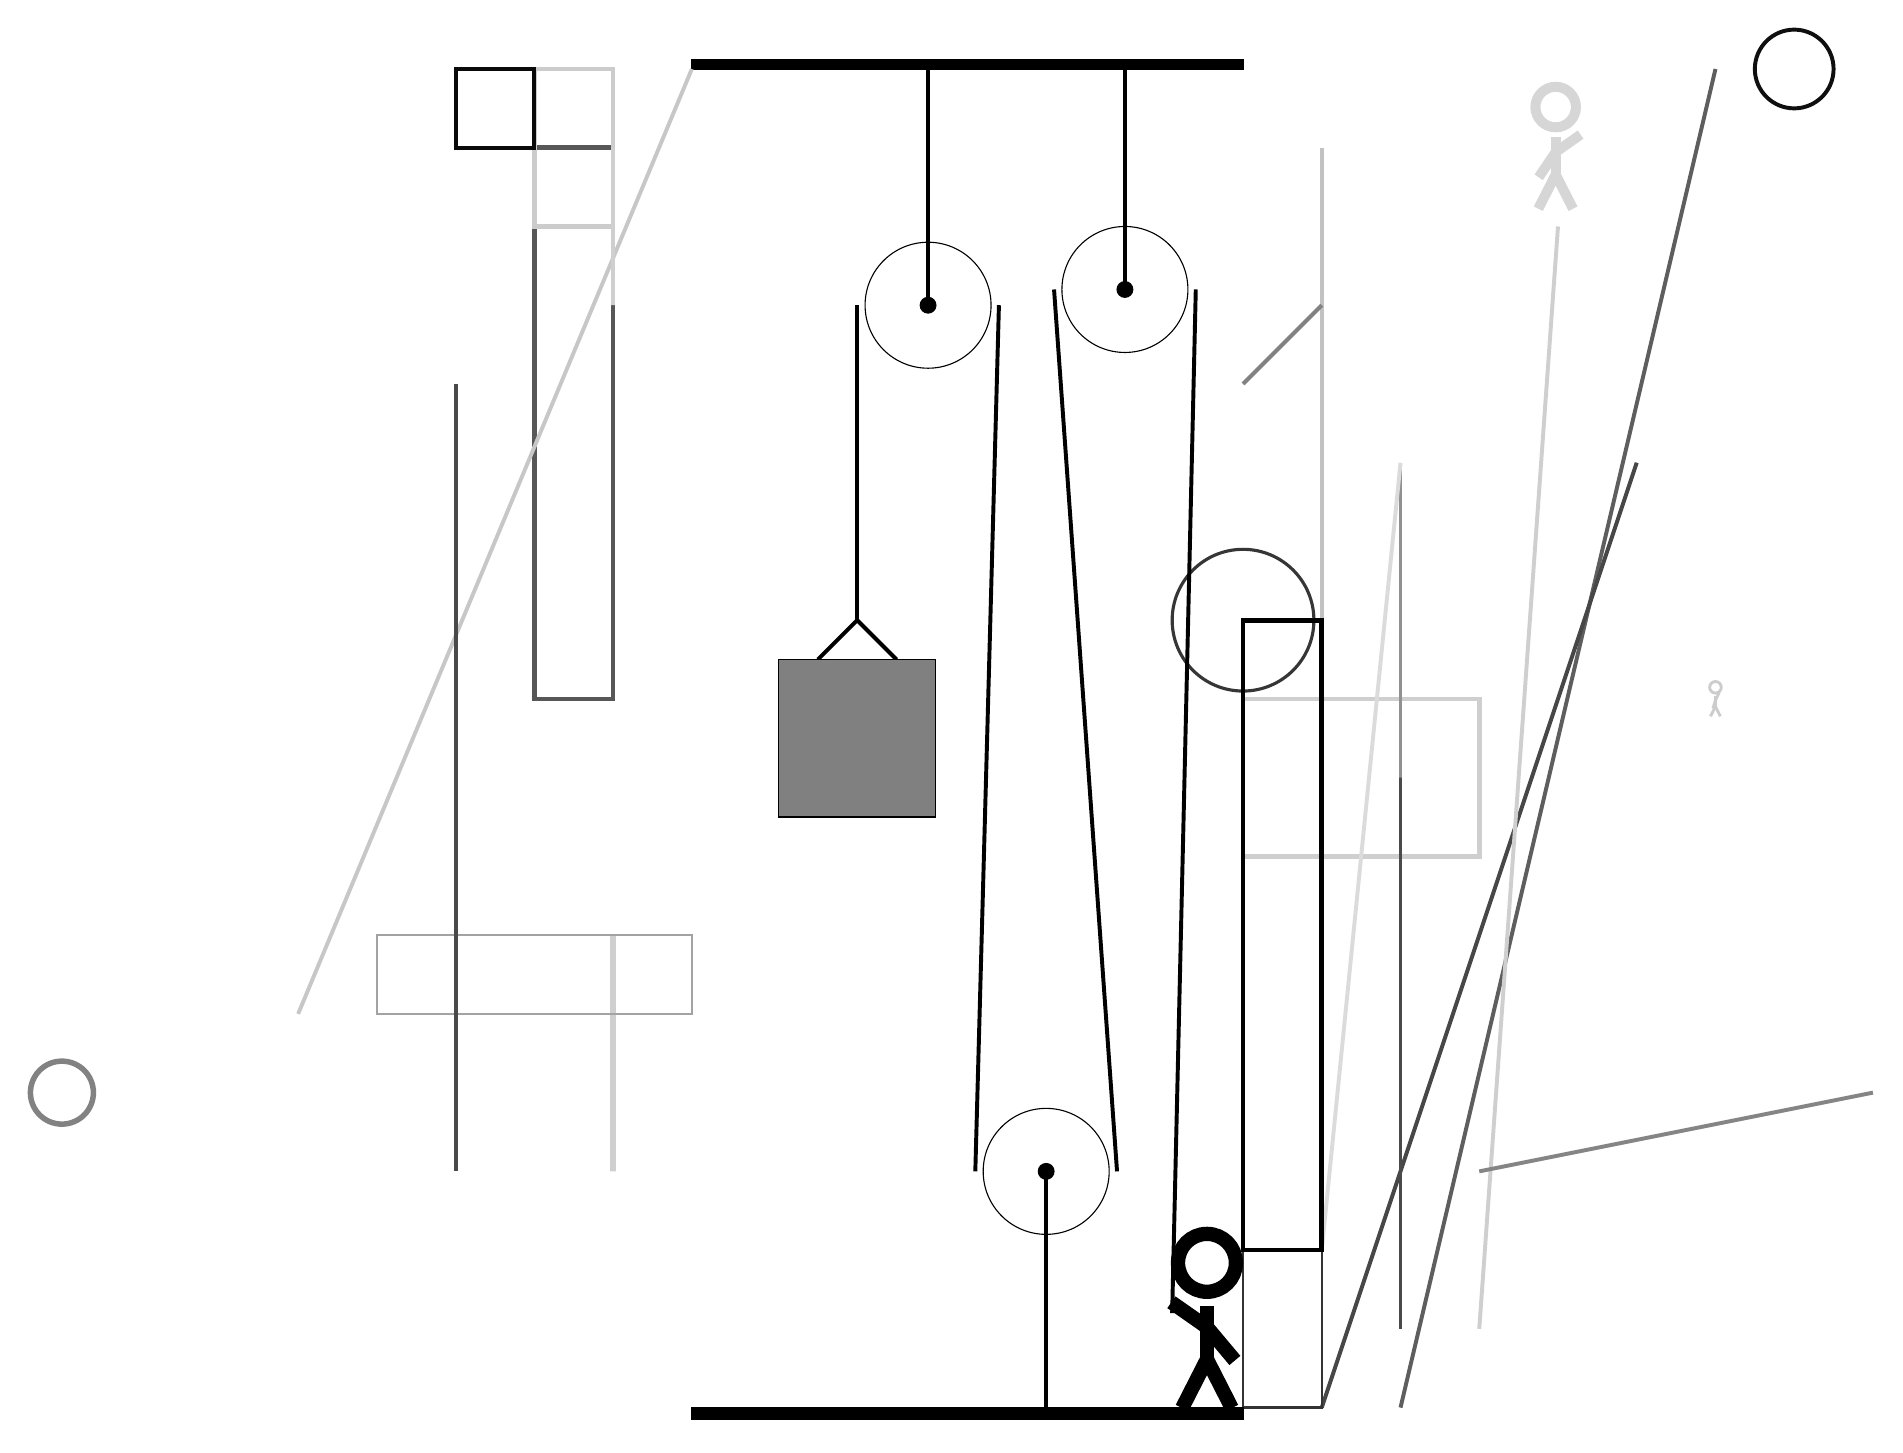
\begin{tikzpicture}
			%%%%% START %%%%%
			
			\draw[fill=black] (-2, 14) rectangle (5, 14.125);
			
			\draw (1, 11) circle (0.8);
			\draw[fill=black] (1, 11) circle (0.1);
			\draw[line width=0.5mm]  (1, 14) -- (1, 11);
			
			\draw[fill=white](2.5, 0) circle (0.8);
			\draw[fill=black] (2.5, 0) circle (0.1);
			\draw[line width=0.5mm]  (2.5, -3) -- (2.5, 0);
			
			\draw[fill=white](3.5, 11.2) circle (0.8);
			\draw[fill=black] (3.5, 11.2) circle (0.1);
			\draw[line width=0.5mm] (3.5, 14) -- (3.5, 11.2);
			
			\draw[line width=0.6mm, color=black!66] (-4, 13) rectangle (-3, 6);
			
			\node[line width=0.7mm, color=black!16] at (9, 13) {\Strichmaxerl[7][56][35]};
			\draw[line width=0.5mm, color=black!24](6, 3) -- (6, 13);
			\draw[line width=0.6mm, color=black!20] (-3, 14) rectangle (-4, 12);
			\draw[line width=0.5mm, color=black!63](7, -3) -- (11, 14);
			
			\draw[line width=0.6mm, color=black!19] (5, 6) rectangle (8, 4);
			
			\draw[line width=0.5mm, color=black!43](7, -1) -- (7, 9);
			
			\draw[line width=0.5mm, color=black!22](-7, 2) -- (-2, 14);
			\draw[line width=0.5mm, color=black!72](6, -3) -- (10, 9);
			\draw[line width=0.5mm, color=black!14](7, 9) -- (6, -1);
			
			\draw[line width=0.3mm, color=black!80] (5, -3) rectangle (6, -1);
			\draw [line width=0.4mm, color=black!79](5, 7) circle (0.9);
			\draw[line width=0.5mm, color=black!19] (-3, 11) rectangle (-3, 13);
			
			\draw[line width=0.6mm, color=black!100] (6, -1) rectangle (5, 7);
			\node[line width=0.2mm, color=black!20] at (11, 6) {\Strichmaxerl[2][73][64]};
			\draw[line width=0.7mm, color=black!19] (-3, 3) rectangle (-3, 0);
			
			\draw[line width=0.5mm, color=black!49](5, 10) -- (6, 11);
			
			\draw[line width=0.5mm, color=black!19](9, 12) -- (8, -2);
			\draw[line width=0.5mm, color=black!71] (7, 5) rectangle (7, -2);
			\draw[line width=0.5mm, color=black!96] (-4, 14) rectangle (-5, 13);
			\draw[line width=0.2mm, color=black!36] (-2, 2) rectangle (-6, 3);
			
			\draw[line width=0.5mm, color=black!71](-5, 10) -- (-5, 0);
			\draw[line width=0.5mm, color=black!48](8, 0) -- (13, 1);
			\draw [line width=0.5mm, color=black!94](12, 14) circle (0.5);
			\draw [line width=0.7mm, color=black!49](-10, 1) circle (0.4);
			
			
			\draw[line width=0.5mm] (-0.4, 6.5) -- (0.1, 7.0) -- (0.6, 6.5);
			\draw[fill=black!50] (-0.9, 6.5) rectangle (1.1, 4.5);
			
			\draw[line width=0.5mm] (0.1, 11) -- (0.1, 7.0);
			\centerarc[line width=0.5mm](1, 11)(0:180:0.9);
			\draw[line width=0.5mm](1.9, 11) -- (1.6, 0);
			\centerarc[line width=0.5mm](2.5, 0)(180:360:0.9);
			\draw[line width=0.5mm](3.4, 0) -- (2.6, 11.2);
			\centerarc[line width=0.5mm](3.5, 11.2)(0:180:0.9);
			\draw[line width=0.5mm](4.4, 11.2) -- (4.1, -1.8);
			
			\node at (4.5, -1.9) {\Strichmaxerl[10][-35][-50]};
			
			\draw[fill=black] (-2, -3) rectangle (5, -3.15);
			
			%%%%% END %%%%%
		\end{tikzpicture}
	\end{figure}	
\end{document}